% Meeting prep for the research advisor: three results and one proposed direction, on one page.
% Numbers from the saved runs (../exp3/LOG.md, ../exp3/ANALYSIS.md); figure from ../exp3/advisor_figure.py.
% Build (from this folder): pdflatex advisor_onepager.tex
\documentclass[10pt]{article}
\usepackage{pifont}
\usepackage[letterpaper,margin=0.5in]{geometry}
\usepackage[T1]{fontenc}
\usepackage[scaled=0.92]{helvet}
\renewcommand{\familydefault}{\sfdefault}
\usepackage{microtype}
\usepackage{xcolor}
\usepackage{graphicx}
\usepackage{enumitem}
\usepackage[hidelinks]{hyperref}
\setlength{\parindent}{0pt}
\setlength{\parskip}{3pt}
\setlist{nosep,leftmargin=1.1em,itemsep=1.5pt}
\definecolor{cblue}{HTML}{2A78D6}
\definecolor{corange}{HTML}{EB6834}
\definecolor{ink2}{HTML}{52514E}
\definecolor{muted}{HTML}{898781}
\definecolor{axis}{HTML}{C3C2B7}
\definecolor{plane}{HTML}{F4F3EF}
\newcommand{\boxed}[1]{\fcolorbox{axis}{plane}{\parbox{\dimexpr\linewidth-2\fboxsep-2\fboxrule}{#1}}}

\begin{document}
\small

{\Large\bfseries When do GPT-2's attention heads rest? Three results and a proposal}\\[1pt]
{\footnotesize\color{muted} Pablo Leyva \,·\, meeting prep \,·\, GPT-2 small, BOS + 32 tokens, attention measured at the final token \,·\, \textbf{resting} = late-layer (6--11) attention parked on the first token (BOS), the candidate no-op \,·\, all predictions pre-registered}

\vspace{4pt}
\boxed{\normalsize\textbf{Summary}\\[2pt]
\textbf{\color{cblue}\ding{172}\,} \textbf{More coherent text $\to$ more resting.} Late heads' BOS attention rises steadily with the amount of natural text before an unrelated final token (+0.13 / +0.16 at 31 tokens, vs random tokens), needs word order, and keeps 65--72\% when the last two words are randomized.\\[2pt]
\textbf{\color{cblue}\ding{173}\,} \textbf{Completion releases it.} When the final token completes the context (a country's capital, a phrase's object, a passage's next word), late heads rest less ($-0.02$ to $-0.06$); for country$\to$capital this held from every one of the 31 positions.\\[2pt]
\textbf{\color{cblue}\ding{174}\,} \textbf{Truth alone does not.} A correct vs wrong country--capital pair before an unrelated final token barely moves resting ($-0.001$ / $-0.004$), though GPT-2 knows all 11 capitals; any real pair raises it (+0.013 / +0.05).\\[3pt]
$\Rightarrow$ \textbf{Working hypothesis:} heads rest when there is coherent context the current token does not use (``nothing to integrate'').}

\vspace{4pt}
\centering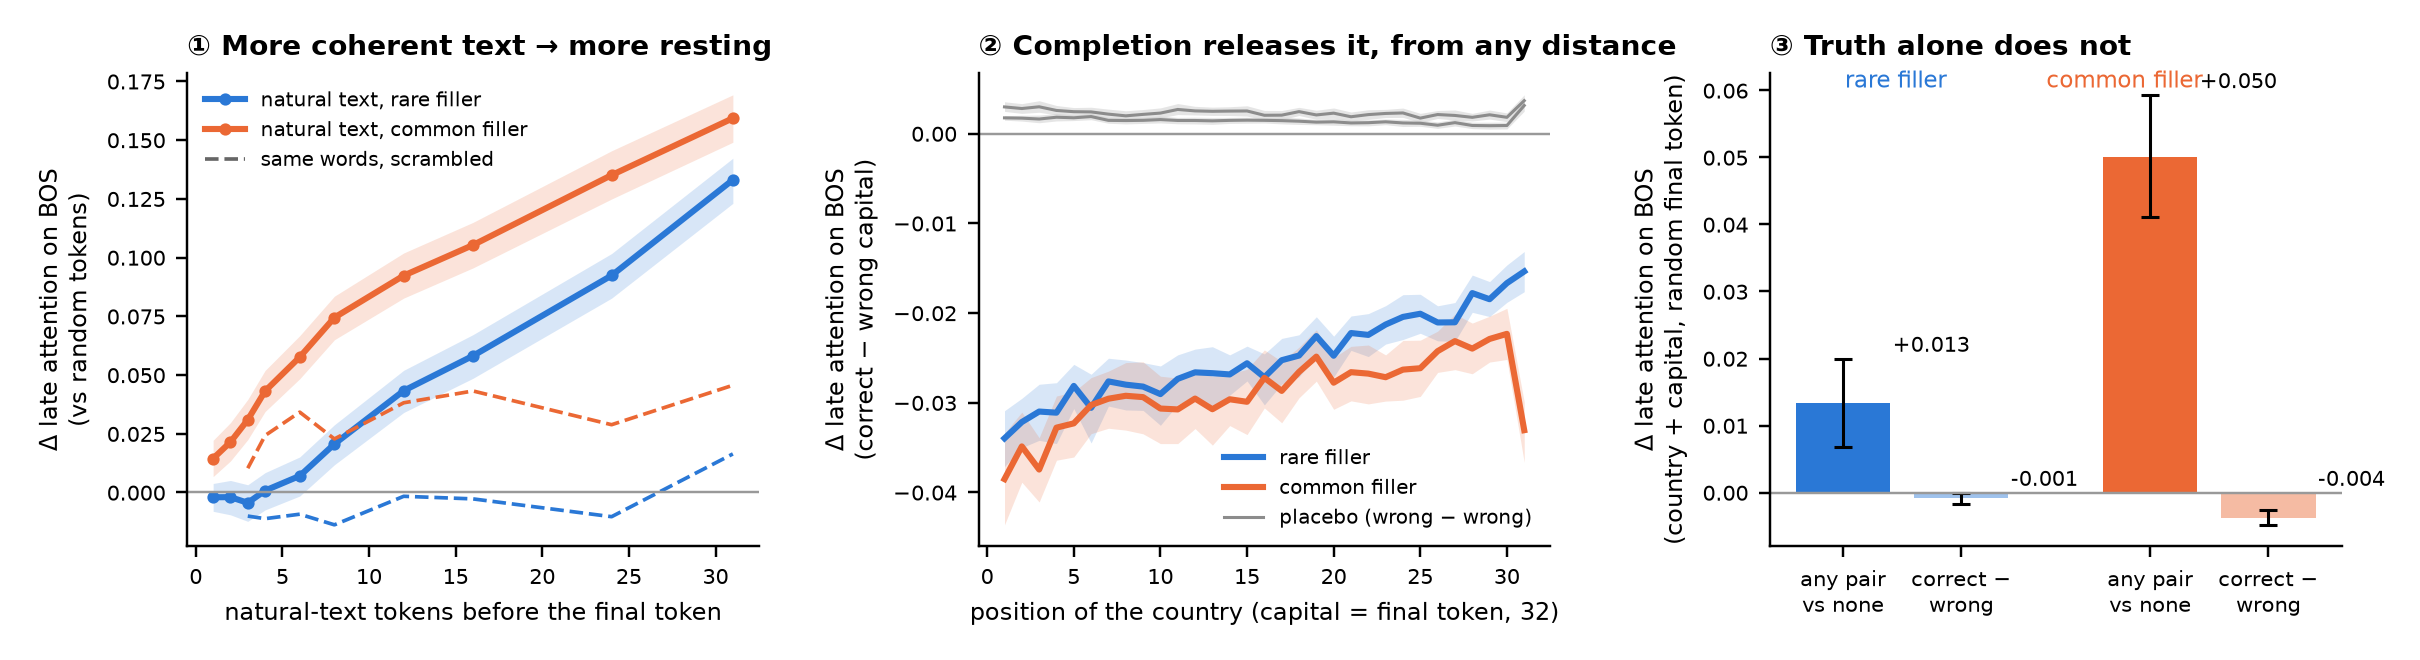
\includegraphics[width=\linewidth]{advisor_fig.png}
\raggedright

{\footnotesize\color{ink2} Blue / orange = rare / common random filler tokens (two independent replications). Bands and bars = 95\% bootstrap CIs over 50--200 rows.}

\vspace{3pt}
\begin{minipage}[t]{0.325\linewidth}\footnotesize
\textbf{\ding{172} How (E3.2).} The last $k$ = 1--31 tokens of 12 hand-written passages before a random final token; 200 rows $\times$ 2 filler types. Controls: the same tokens scrambled, and same-form random words. 12/12 passages positive from $k$ = 12. Overturns our earlier ``last word pair'' account, which held only for 3-word phrases.
\end{minipage}\hfill
\begin{minipage}[t]{0.325\linewidth}\footnotesize
\textbf{\ding{173} How (R1-in + sweep).} Every country paired with every capital, so each capital is the final token once correctly and ten times wrongly: token identity cancels in correct $-$ wrong. Adjacent: $-0.018$ / $-0.034$, 11/11 countries, permutation $p < 10^{-4}$. Same direction for cities, phrase objects ($-0.03$ to $-0.05$) and natural next words ($-0.06$, 12/12 passages).
\end{minipage}\hfill
\begin{minipage}[t]{0.325\linewidth}\footnotesize
\textbf{\ding{174} How (R1-out).} Same grid with the pair at 30--31 and a random final token. Manipulation check: at the country, GPT-2 prefers its own capital in 11/11 countries (+2.4 / +2.7 nats). The pairing shows up elsewhere: correct pairs shift attention inside the pair from the capital to the country.
\end{minipage}

\vspace{4pt}
{\footnotesize\textbf{Why trust it:} TransformerLens and Hugging Face agree to $<5\times10^{-5}$; reruns are bit-identical; placebo contrasts flag $\le$1 head (0 of 496 sweep placements); a positive control works (known induction heads L5H5, L6H9 switch from BOS to the copy target); 19 of 37 pre-registered predictions held, and the failures are reported. \textbf{Limits:} GPT-2 small only; random-token contexts except E3.2; some effects differ between the two filler types.}

\vspace{5pt}
\boxed{\textbf{Proposed next direction: is resting actually a no-op?}\\[2pt]
\textbf{Why this, causally.} \ding{172}--\ding{174} show that BOS attention tracks whether the current token has context to integrate, but every result so far is an \emph{attention weight}; ``no-op'' is still an interpretation. The results also hand us the tool to test it: \ding{172} and \ding{173} are two dials that move resting in opposite directions while holding the tokens fixed (amount of coherent text; correct vs wrong completion with the same final token). So we can change resting without changing the input tokens, and ask whether the computation changes with it.\\[2pt]
\textbf{Test.} (1) \emph{Value-weighted attention:} does a resting head's output ($\sum_k \alpha_k v_k$) shrink toward zero as its BOS weight rises? (2) \emph{Ablation:} mean-ablate each late head and measure the change in the model's next-token distribution (KL) in high-resting vs released contexts from the same grids.\\[2pt]
\textbf{Prediction and stakes.} A no-op predicts near-zero output and near-zero ablation cost while heads rest, and a larger cost once completion releases them. Confirmed, ``resting = no-op'' becomes a measured property and \ding{173}'s completion signal becomes the target for circuit work (patching what tells late heads to stop resting). Refuted, BOS attention does real work and the thesis has to change.}

\end{document}
